
Based on our specification we have created a design for the application's user interface (UI). The UI had to support the use cases specified in section \ref*{sec:use_cases}. In the MoSCoW analysis we specified a ranking of features from the use cases in order of \textit{must have}, \textit{should have},\textit{could have} and \textit{wont have}. In the design we prioritized the features listed in the \textit{must have} category, however we have also accounted for features listed in other categories. The two features \textbf{Students can retrieve exercises descriptions} and \textbf{Students can submit exercise attempts}, listed in the \textit{must have} category corresponds to the use case \textit{Solve exercises}.
In figure \ref{fig:wfExercise} the wire-frame design that satisfies the use case.
% primary use cases
% solve exercises
\begin{figure}[H]
	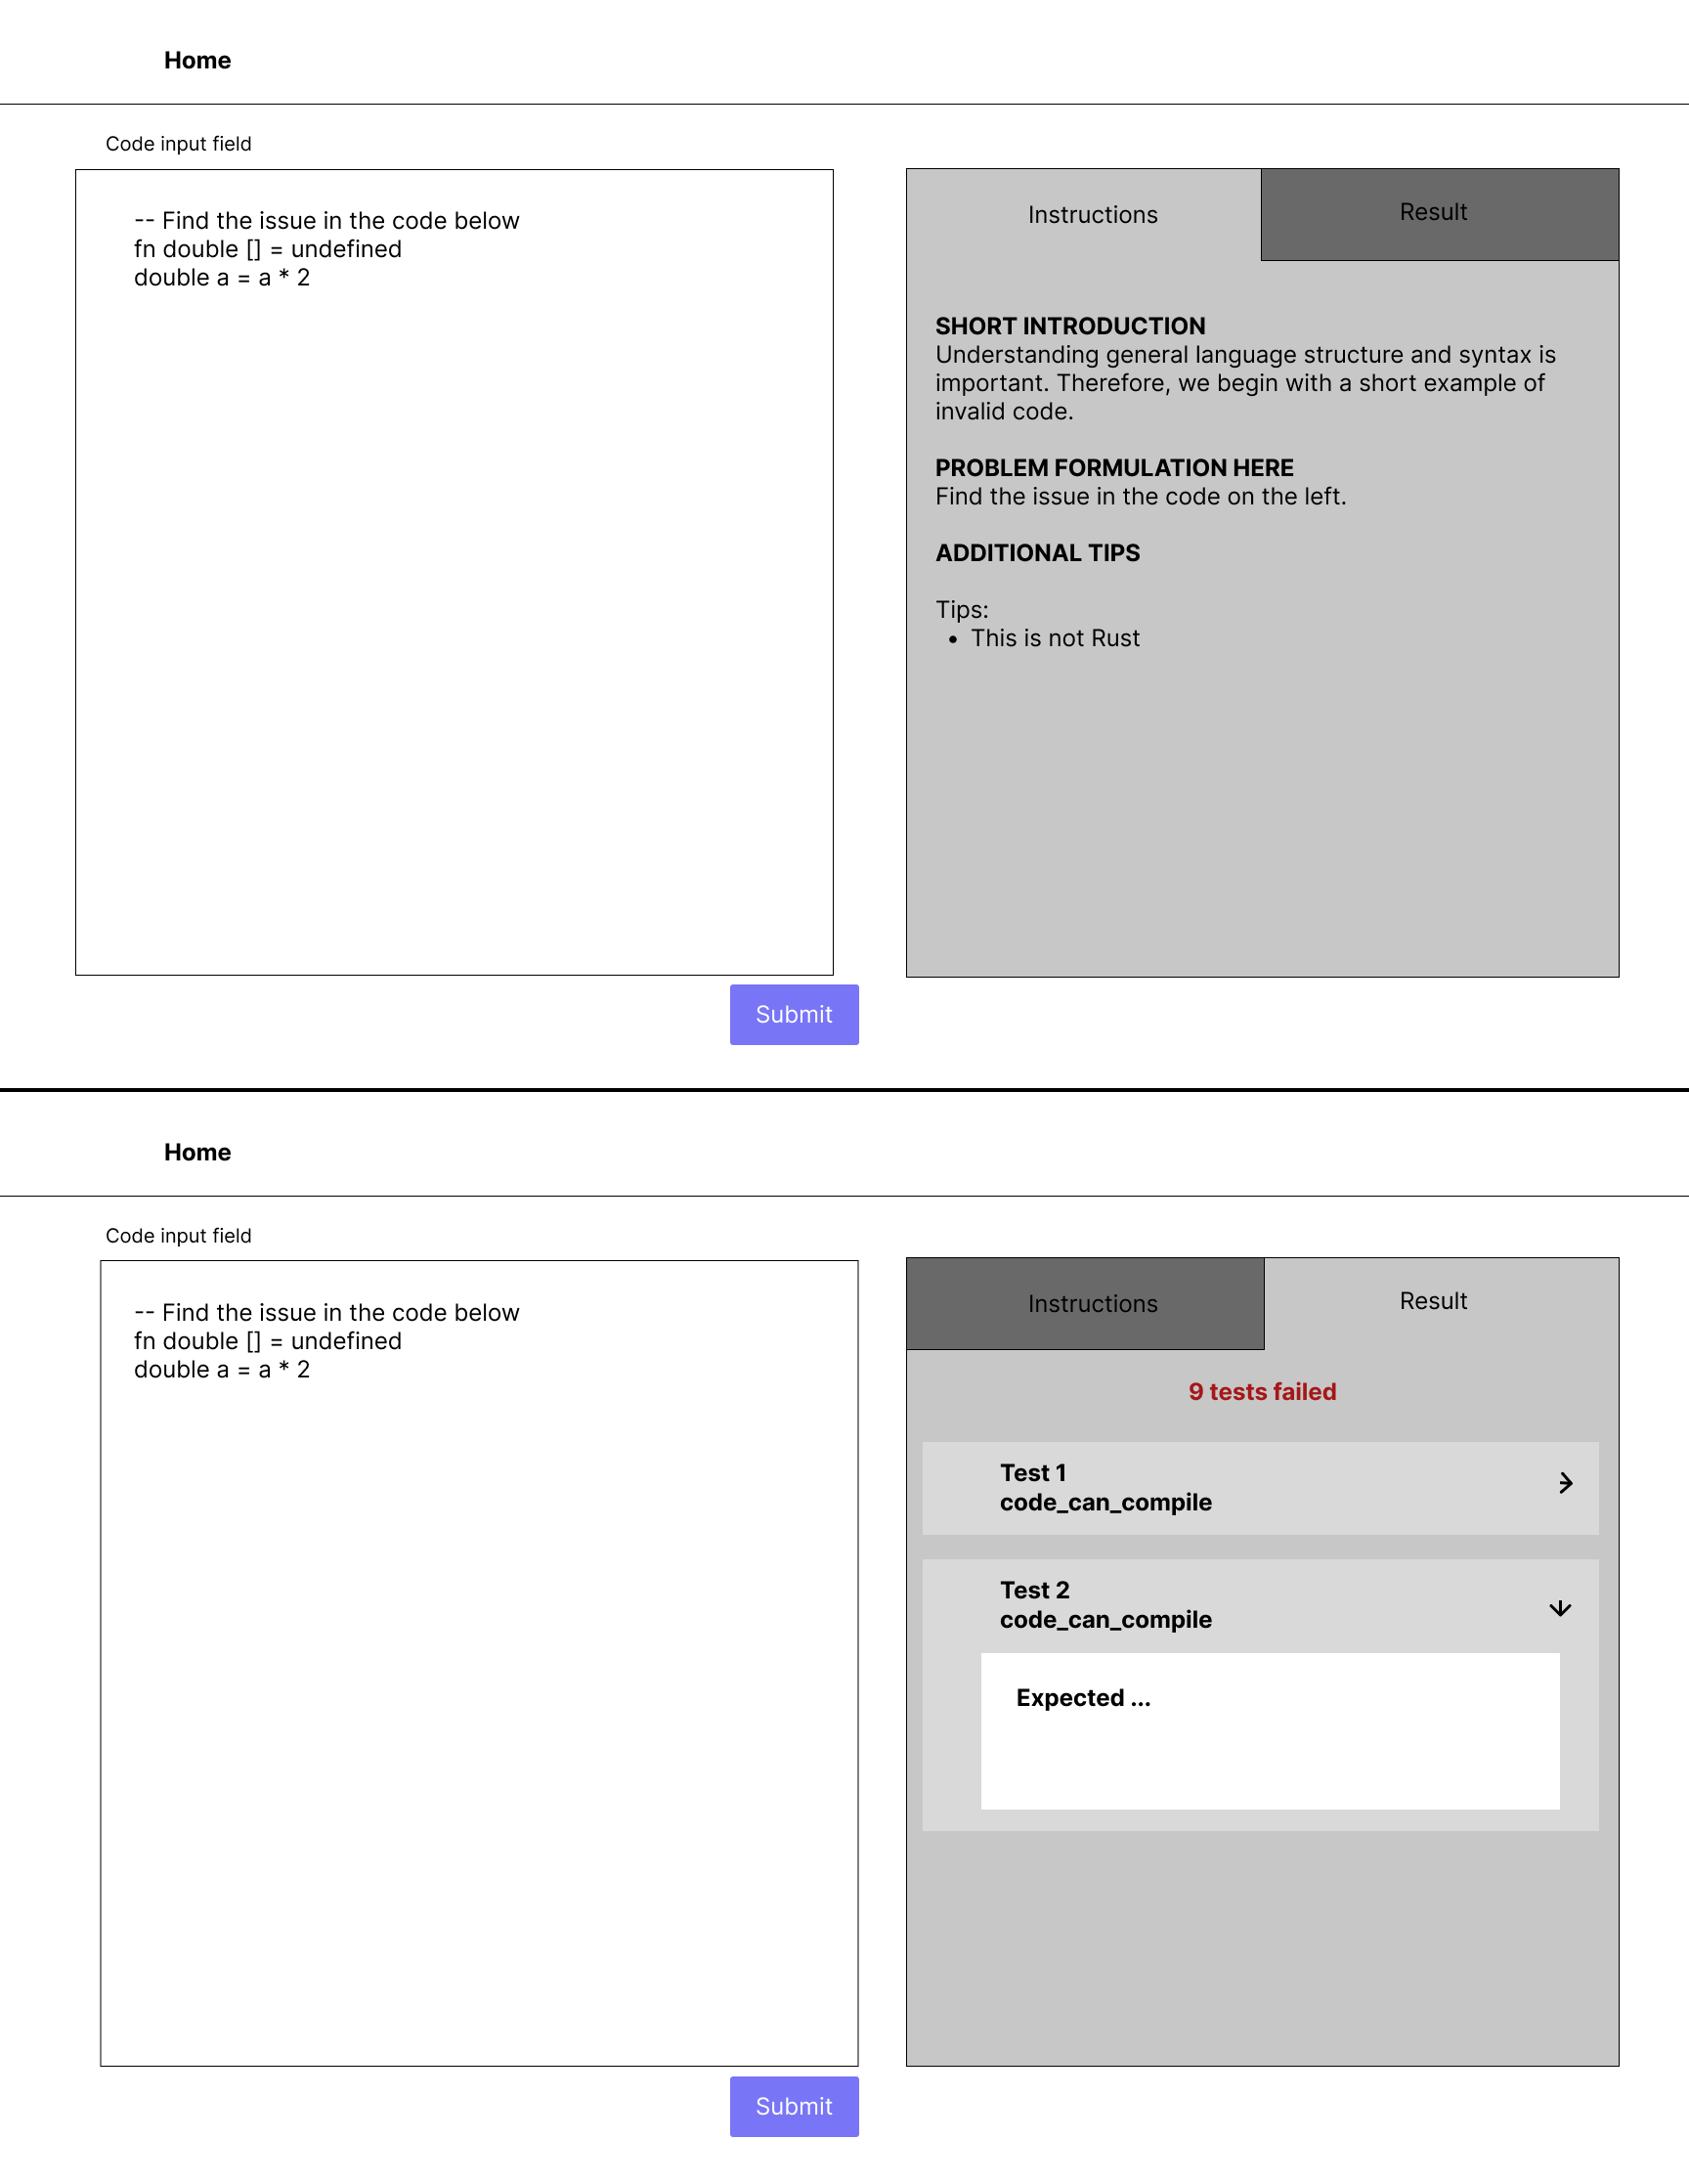
\includegraphics[scale=0.6]{WireframeSolveExercise.png}
	\centering
	\caption{wireframe for solving an exercise}
	\label{fig:wfExercise}
\end{figure}

For both images in figure \ref{fig:wfExercise} a text input field can be seen located on the left. This text input field is where the user can input code for submission. On the right side of the left-most image of figure \ref{fig:wfExercise}, a box can be seen containing two tabs. The currently selected tab of this image is the \textit{Instructions} tab which is where the instructions for the current exercise is displayed. On the right ride of the right-most image is a similar view, except that the \textit{Result} tab has now been selected. This tab shows the result of the submitted code, whether it passed the tests for the exercise and whether it compiled. This satisfies the requirements that an exercise should have a description and that a user should be able to submit and verify their code and exercise submission stated in the \textbf{Use case: Solve exercises}.

The page displayed in figure \ref{fig:wfExercise} does not satisfy the entirety of the use case \textbf{Use case: Solve exercises}, as we have designed a separate page to browse exercises as well as sessions and syllabi. The page structure for all of these are similar, and therefore we only show an example of a page for browsing syllabi.
% Structure of creating sessions and syllabi
\begin{figure}[H]
    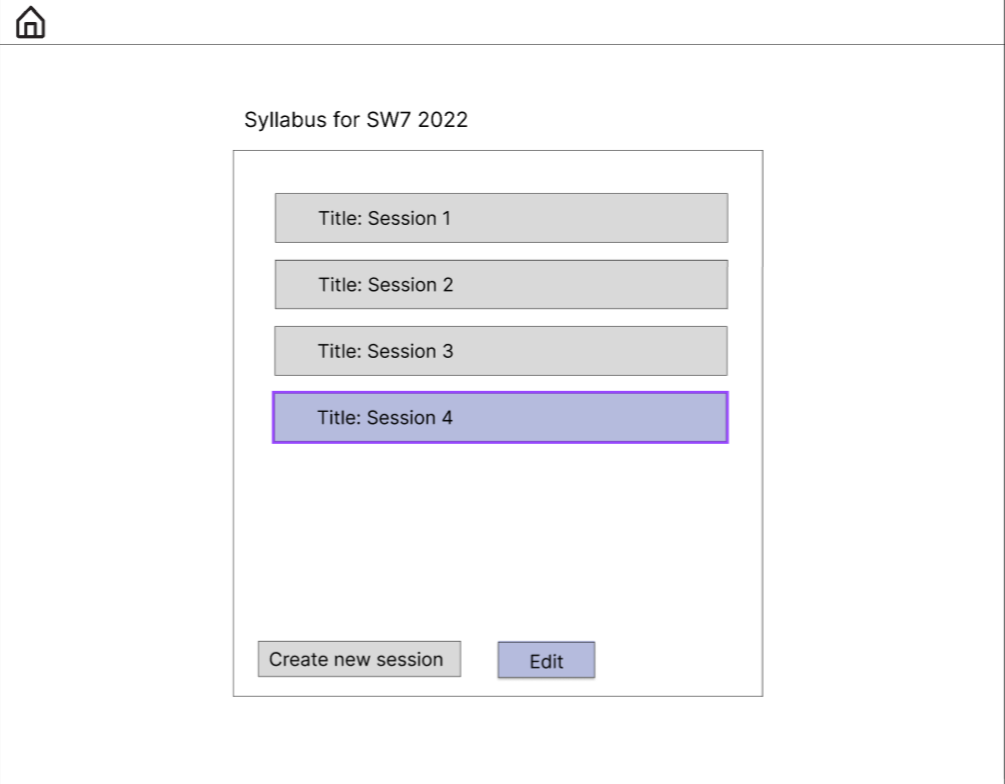
\includegraphics[scale=0.6]{browseSyllabus.png}
    \centering
    \caption{wireframe for browsing a syllabus}
    \label{fig:wfSyllabus}
\end{figure}
Note that the buttons related to creating new items or updating items in the list will only be available to the lecturer. The items shown in the list corresponds to which page that the user is on. If the user is browsing syllabi, then the items contained in the list will be syllabi. If the user is browsing sessions, the list will contain sessions. Similarly for exercises.
% create exercises
\begin{figure}[H]
	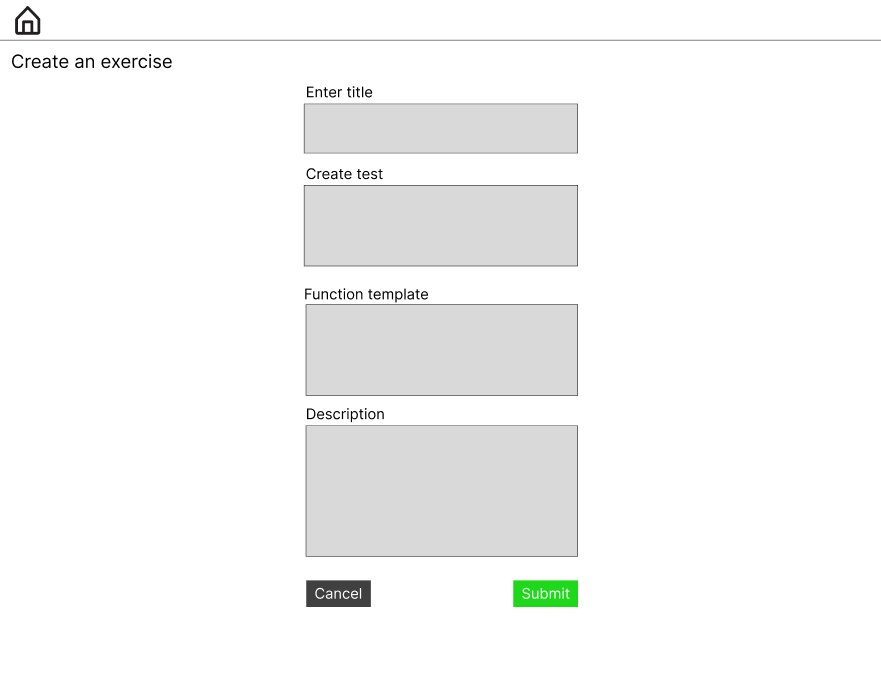
\includegraphics[scale=0.6]{createProblem.jpg}
	\centering
	\caption{wireframe for creating a problem}
	\label{fig:wfProblem}
\end{figure}


% secondary
% view solutions
% account use case